\documentclass[9pt, oneside]{article}   	% use "amsart" instead of "article" for AMSLaTeX format
\usepackage[left=2cm, right=2cm, top=3cm]{geometry}
\usepackage{cite}
\usepackage[english]{babel}
\usepackage{geometry}                		% See geometry.pdf to learn the layout options. There are lots.
\geometry{letterpaper}                   		% ... or a4paper or a5paper or ... 
\usepackage{graphicx,kantlipsum,setspace}
\usepackage{caption}			% Use pdf, png, jpg, or eps§ with pdflatex; use eps in DVI mode
\captionsetup[table]{font={stretch=1.15}}     %% change 1.2 as you like
\captionsetup[figure]{font={stretch=1.15}} 
\graphicspath{ {images/} }		% TeX will automatically convert eps --> pdf in pdflatex
\PassOptionsToPackage{hyphens}{url}\usepackage{hyperref}
\renewcommand{\UrlFont}{\small\tt}
\usepackage[euler]{textgreek}
\usepackage{verbatim}						
\usepackage{titlesec}
\titlelabel{\thetitle.\quad}
\usepackage{amssymb}
\linespread{1.15}
\usepackage{gensymb}
\usepackage{textcomp}
\usepackage{setspace}
\usepackage[symbol]{footmisc}
\usepackage[version=4]{mhchem}
\usepackage{multicol}
\setlength\columnsep{20pt}
\usepackage{wrapfig}
\setlength{\parindent}{1cm} % Default is 15pt.
\usepackage{oz}
\usepackage{makecell}  

\usepackage{longtable}

\usepackage[ruled,lined,linesnumbered,noresetcount,shortend]{algorithm2e}
\SetKwFor{For}{for (}{) }{end}
\SetKwFor{lineToEnd}{...}{}{end}
\SetKwFor{Loop}{Loop}{}{EndLoop}
\SetKwBlock{contIndent}{...}{}
\let\oldnl\nl% Store \nl in \oldnl
\newcommand{\nonl}{\renewcommand{\nl}{\let\nl\oldnl}}% Remove line number for one line




% 2 is subsection, 3 is subsubsection
\setcounter{tocdepth}{3}
\setlength{\parindent}{.5 cm}

\begin{document}
\newpage


\begin{center}
\Large{\textbf{Data Provenance Over Computational Graphs}}
\vspace{1 cm}

\normalsize{}
Alan Ransil

Protocol Labs

alan@protocol.ai

\vspace{1 cm}
Updated \today

\vspace{1 cm}
\Large{\textbf{Abstract}}

\end{center}

\noindent Data-driven decision making requires combining trusted information from many sources. Here, we introduce two protocols which together allow end-to-end tracing of data provenance over computational pipelines. The first protocol, Transform.Storage, models pipelines as symmetric monoidal categories anchored in content-addressed data types. This allows both reproducible and non-reproducible real-world processes to be described as accessible wiring diagrams. Secondly, the Provenance Protocol uses signatures over data and code to evaluate trust with respect to a community.  While the two protocols may be used independently, together they form a three-layer system dynamically tracing data provenance. To the extent that trust is compositional, this allows a rigorous examination of the flow of trust through through complex and multi-party computational processes. We explore applications of this paradigm to real-world use cases.



\setlength{\parskip}{0.1\baselineskip} %Controls vertical space between paragraphs, can re-set line by line
\section{Introduction}

There is a need to establish the end-to-end reasoning behind data driven decisions, and in particular reasoning incorporating data supplied by many parties. Several trends make this need increasingly urgent. First, the trend towards using public and open source data to substantiate decisions increases the utility of expressing these decisions using transparent end-to-end compute pipelines. Second, decisions are increasingly automated with IOT, smart contract and AI subsystems forming parts of the decision making pipeline. Explicitly recording this pipeline is necessary to substantiate trust in the end result. Third, generative AI heightens the need to rigorously track the provenance of data to combat misinformation. Fourth, decisions in critical areas such as environmental sustainability and AI ethics and safety rely on rapidly evolving research which carries an imperative to explicitly lay out methodologies so that they can be reproduced, challenged, improved, and rapidly applied. Fifth, the introduction of more powerful and general zero knowledge systems increases the necessity of tracing decisions end-to-end so that proven claims relying on little revealed information can be put into context.

Here we introduce two protocols that together can be used to model end-to-end decisions as modular compute pipelines, reproduce their results if sufficient information is revealed, establish trust relative to norms determined by user communities, and allow subsequent users to reuse or extend these pipelines without sacrificing verifiability. These protocols model compute pipelines in three layers as shown in figure \ref{layeredDataFig1}. The first protocol, Transform.Storage, represents functions as modular, directional relationships between data types. At the data Asset layer, this defines pipelines as typed datasets on a two-dimensional grid along with functional maps between them. At the Function layer, Transform.Storage represents function definitions coupled with input and output types. The correspondence between these layers is determined by the types of Assets on the lower level and the input and output types of Functions at the middle level. The second protocol, the Provenance Protocol, can be used to apply provenance information to data, functions and pipelines and define bounded trust in each relative to community norms. While the two protocols can be used separately, together they can be used to automatically map the flow of trust evaluated relative to a given Provenance community.

\section{Previous Work}\label{PrevWork}

This section does not attempt a comprehensive literature review of relevant projects. Included are brief descriptions of some of the work which inspired our approach, highlighting some critical differences in design decisions.

\subsection{Decentralized Identifiers and Verifiable Credentials}\label{did-vc}

The World Wide Web Consortium (W3C) developed standards for Decentralized Identifiers (DIDs) and Verifiable Credentials (VCs) to allow management of identities and credentials without a centralized registry. Following these standards, a self-sovereign DID may be generated for an individual or organization. The DID controller establishes and signs a DID Document which describes the public keys, authentication and delegation protocols, and endpoints associated with the DID. By separating the DID Document from the controller's key pair, this specification enables a persistent self-sovereign identifier that supports method upgrades and key pair rotation. \cite{w3cDID}

\begin{center}
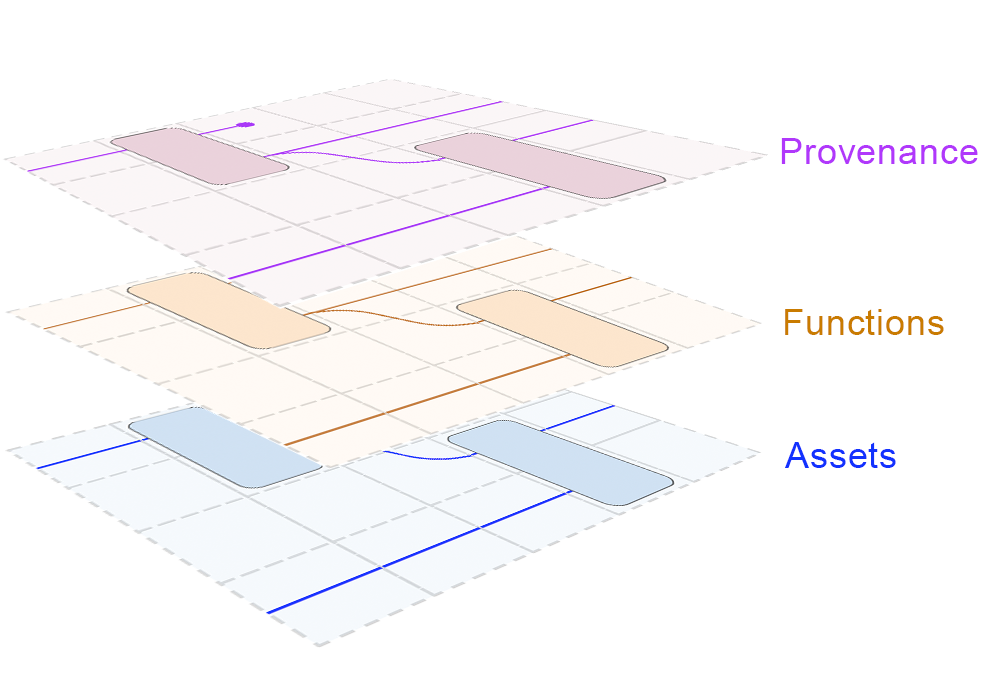
\includegraphics[width=0.5\columnwidth]{Fig1_assets_20230715}
\begin{flushright}
\captionof{figure}[Three layers of a compute pipeline]{The three layers of a compute pipeline include underlying data assets, functions operating on those assets, and provenance establishing the origins of the lower two layers. Data types establish a correspondence between the asset and function layers, while provenance metadata operating over the lower two layers establishes a flow of trust.}
\label{layeredDataFig1}
\end{flushright}
\end{center}

\subsection{IPFS}\label{IPFS}
Tracing decisions end-to-end requires interoperating between work done by many individuals on many different computers and subsystems. The protocols typically used to communicate between machines, such as TCP and https, operate on the basis of location addressing. Under this design pattern, information does not have a persistent identifier and interoperability typically relies on centralized services maintaining endpoints which resolve to network locations. Users of these services typically do not control their own key pairs, which disintermediates them from their data. While the results of these design decisions on market power and centralization of economic control are widely discussed, their implications for data management are similarly profound. Because users are expected to rely on companies to maintain the integrity of their data and market incentives induce vendors to lock in users, it is difficult for developers to write code that traces data across the boundaries between software subsystems.

The Interplanetary File System (IPFS) is a protocol which allows users to address and deliver content based on the cryptographic hash of that content rather than its location on the network \cite{ipfs-paper}. This design pattern, namely using a content address as a URI rather than a location address, is essential for maintaining interoperability and will therefore be used as the basis for data addressing in this work.


\subsection{Wiring Diagrams and Symmetric Monoidal Categories}\label{smc}

Wiring diagrams are computational graphs in which data types are represented by lines and functions are represented by boxes. It has been shown that they can be interpreted rigorously as representations of symmetric monoidal categories (SMCs). \cite{Patterson_2021} 


A category is a mathematical structure containing objects as well as directional relationships between objects known as morphisms. Morphisms must compose, meaning that if morphisms $f : A \rightarrow B$ (morphism $f$ is a directional relationship from object $A$ to object $B$) and $g : B \rightarrow C$ both exist in a category then there must also exist $h : A \rightarrow C$ such that $h = f \zcmp g$. A monoidal category is a category with a product operation, ie. $(A \otimes B)$. 

A SMC is a monoidal category with a braiding operation $Braid_{A,B} : A \otimes B \rightarrow B \otimes A$ that is symmetric: $Braid_{A,B} \zcmp Braid_{B,A}=Identity_{A \otimes B}$. If objects in a category are interpreted as data types and morphisms as functions mapping from one datatype to another, then the product in an SMC can be interpreted as an ordered set of two non-interacting data types. 

Representing data pipelines in transform.storage as wiring diagrams is provides a formal grounding for computational diagrams that behave intuitively. The type structure makes it possible to define which functions are allowed to be composed with other functions, and by anchoring types using content addresses we are able to achieve interoperability between data storage and compute platforms without sacrificing verifiability. Furthermore, \textbf{composition and data provenance together allow a rigorous and automatic assessment of the flow of trust through a compute pipeline.}  However, while types in transform.storage should be interpreted strictly composition should not be. In practice, user functions may not be defined over their entire domain (therefore, using the example from above, $h : A \rightarrow C$ such that $h = f \zcmp g$ might not be defined for all values of type $A$) and may not be deterministic or even formally defined themselves. This means that while pipelines and their component functions are interpreted as morphisms within SMCs, compositionality may be broken when the computation is carried out. 

\section{Transform.Storage Data Model}\label{transformtypes}

Here, we describe the type structure and data primitives of transform.storage as of the current protocol version.

\subsection{Data}\label{data}

Any data blob is a valid member of the data layer in transform.storage. It must be content addressed, allowing it to be verified regardless of the system it is stored in. While the protocol may interpret data blobs (as data conforming to a schema, a schema itself, a function, etc), the contents of data blobs are not legible to the protocol.

\subsection{Type}\label{type}

As in type theory, a type in Transform.Storage is a collection of terms sharing a defined set of properties. These may be primitive types such as $string$ and $integer$, or more complex constructed types such as that defined by a data schema. If term $a$ is of type $A$, we express this membership as $a:A$. In general, a given dataset may be a term of multiple types.

Types are expressed in Transform.Storage as either (1) IPLD objects with the canonical attributes described in Table \ref{typeFields}, or (2) logically equivalently, the CIDs of these IPLD objects. Individual implementations may add optional fields.

\begin{center}
\begin{tabular}{ || p{5cm} | p{9cm} ||}
\hline			
\multicolumn{2}{|| l ||}{\textbf{Type Fields}} \\
\hline
\makecell[l]{\textbf{cid} \\ \textit{(CID)}} & \makecell[l]{CID of the data defining this type; for example the CID \\of a schema. May be null.}\\
\hline
\makecell[l]{\textbf{type\_checking} \\ \textit{(string)}} & \makecell[l]{A value from the Type Checking Table, specifying \\ the function $f_{check}$} \\
\hline
\makecell[l]{\textbf{creator} \\ \textit{(string)}} & \makecell[l]{The public identifier of the creator of this type} \\
\hline
\makecell[l]{\textbf{creator\_id\_format} \\ \textit{(string, required if} \textit{Type.creator is} \\ \textit{non-null})} & \makecell[l]{Value from the Identifier Table (section \ref{transformID}) describing \\ the type of identifier associated with the creator \\ field.} \\
\hline
\makecell[l]{\textbf{protocol\_name} \\ \textit{(string)}} & \makecell[l]{Must be ``transform.storage"} \\
\hline
\makecell[l]{\textbf{protocol\_version} \\ \textit{(string)}} & \makecell[l]{The version of the protocol which this type is pursuant \\ to, such as  ``2.0.0"} \\
\hline
\makecell[l]{\textbf{name} \\ \textit{(string, optional)}} & \makecell[l]{Short human-readable label} \\
\hline
\makecell[l]{\textbf{description} \\ \textit{(string, optional)}} &\makecell[l]{ Longer human-readable label}  \\
\hline  
\end{tabular}
\end{center}
 
\captionof{table}[Type Fields]{Definitions of the canonical fields describing a Transform.Storage type.}
\label{typeFields}
\setlength{\parindent}{.5 cm}
\vspace{.25 cm}

The value of $type\_checking$ is cross-referenced with the type checking table maintained at the Transform.Storage spec \cite{transformSpec}, to determine the function $f_{check}$ with the type signature $f_{check}$: $(Type \otimes Data) \rightarrow \{result: Boolean, code: Str\}$. Here, $result$ is true if the input $Data$ is a term of the input $Type$ and false otherwise. The output key $code$ contains an error code, or $null$.

Membership in a type is defined by the fields $cid$, and $type\_checking$. A simple type is defined by the data in $cid$ and the function determined in $type\_checking$ (Figure \ref{typesAssets_fig}a). Alternatively, a series type is represented as an array of the CIDs of types (Figure \ref{typesAssets_fig}b). 


\begin{center}
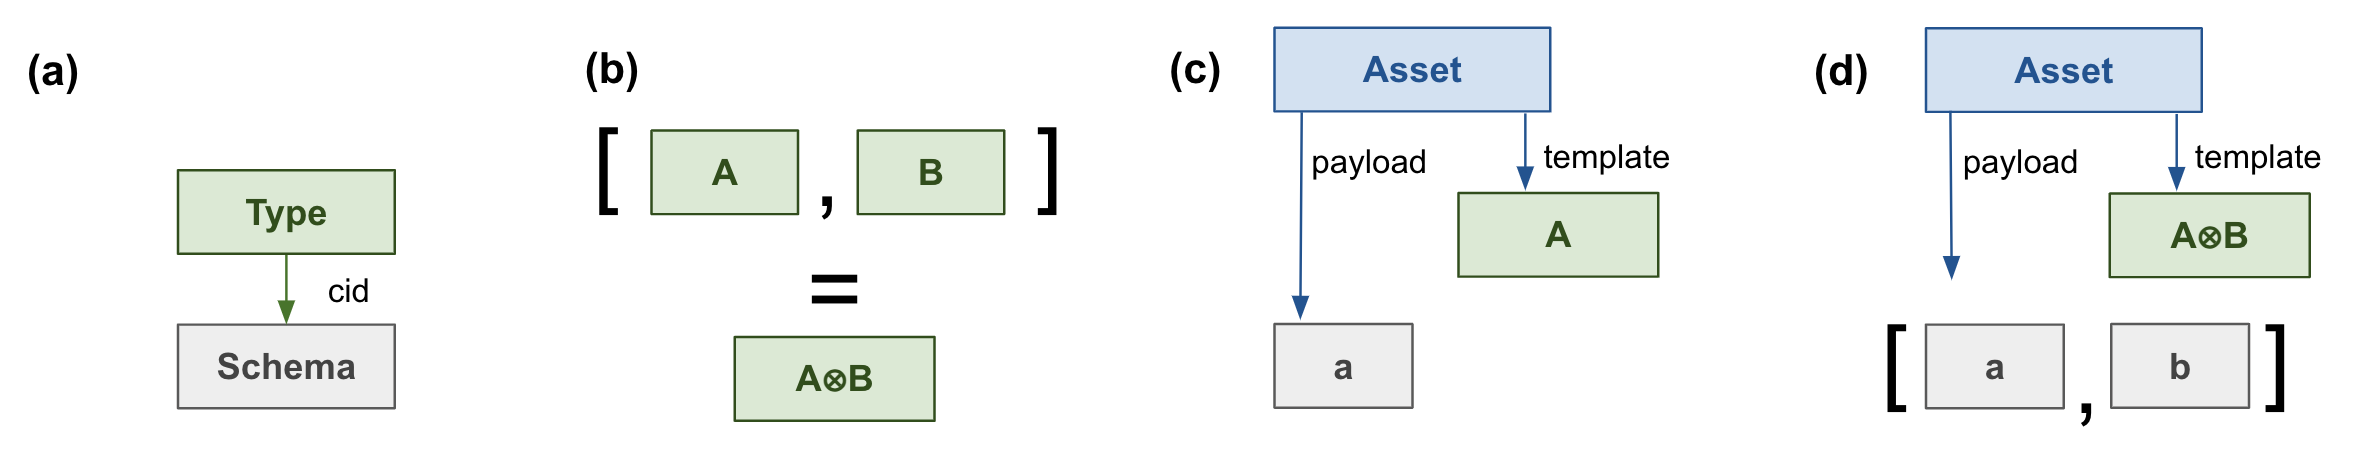
\includegraphics[width=1\columnwidth]{fig_types_assets_20230802}
\captionof{figure}[Types and assets]{Block diagram showing types and assets in Transform.Storage. Blocks represent IPLD objects, (logically equivalently) CIDs of IPLD objects, or CIDs of data blobs and arrow labels represent keys of objects. Brackets represent IPLD arrays. (a) This simple type is defined by a schema which is referenced in its Type.cid field. (b) The series type $A \otimes B$ is represented as an array of the CIDs of types $A$ and $B$, and is logically equivalent to the CID of that array. (c) An asset $a : A$. (d) A series asset, showing $[a, b] : A \otimes B$.}
\label{typesAssets_fig}
\end{center}

Any of the following may thus represent a type:
\begin{enumerate}
\item An IPLD object with the fields in table \ref{typeFields}, representing a simple type
\item An IPLD array in which values are types, representing a series type
\item The CID of any type; logically equivalent to that type
\end{enumerate}


According to the definition given, types may have complex hierarchical structures which mix objects, arrays, the CIDs of objects, and the CIDs of arrays. However, types may be represented in a normal form by obeying the following rules recursively:

\begin{itemize}
\item Expand every type CID: $CID_A \rightarrow A$
\item Expand every CID representing an array: $[..., CID_{[A,B,C]}, ...] \rightarrow [..., [A,B,C], ...]$
\item Promote the contents of every nested array: $ [..., [A,B,C], ...] \rightarrow [..., A,B,C, ...]$
\end{itemize}

This will result in either a single IPLD object in the case of a simple type, or an array of IPLD objects in the case of a series type. Pseudocode for normalizeType is given in Algorithm \ref{algo_isSimpleTypeNormalForm}.

The $height$ of a type is 1 in the case of a simple type, or the \textit{length of the normal form} of a series type.

The CID of an array of types is logically equivalent to that array, $CID_{A \otimes B} = [CID_A, CID_B]$ as shown in figure \ref{typesAssets_fig}b. The CID of an IPLD object is also logically equivalent to that object, so that $CID_{A \otimes B} = A \otimes B$ and $[CID_A, CID_B] = [A,B]$. Note, however, that  if the schema of Type $C$ defines an array consisting of the schemas of $A$ and $B$, this logical equivalence is broken because the protocol does not assess the contents of type schemas. In this situation, we have $\forall [a,b] : A\otimes B,  [a,b] : C$ but $ A\otimes B \neq C$.

Additionally, $True$ and $null$ are simple types. For every data blob $d$, $d : True$. Type $null$ has no terms.

Every implementation of transform.storage must include the function isTerm (Algorithm \ref{algo_isTerm}), which determines whether a data blob is a term of a given type.

\subsection{Asset}\label{asset}

An asset is a data structure asserting that a given dataset is a term of a given type. An asset contains the canonical fields shown in table \ref{assetFields}.

The block diagrams shown in figure \ref{typesAssets_fig} express (c) $a : A$, and (d) $[a, b] : A \otimes B$. 

The type referenced by $Asset.template$ does not need to be in a normal form as described in section \ref{type} and there are many equivalent representations of any given type. However, the data referenced by $Asset.payload$ is more restricted in that payload CIDs are not hierarchically resolved by the protocol. Thus, if $Asset.payload$ is a CID then either the normal form of $Asset.template$ must be a simple type, or the $Asset.payload$ CID must resolve to an array of data elements matching the $Asset.template$ series type. If $Asset.payload$ is an array then the normal form of $Asset.template$ must be an array with the same number of elements, or $Asset.template$ must be a simple type describing an array. Further hierarchical layers of $Asset.payload$ are not resolved. This is because, while the protocol constrains the structure of types, the contents of data blobs are exogenous to the protocol. If this were not the case, and asset payloads were allowed to contain hierarchical structures similar to series types, it would in principle be impossible for the protocol to distinguish the nested structure of the payload from any underlying structure of the payload data without constraining the structure of that data. This would violate non-interference (section \Ref{nonInterference})
\setlength{\parindent}{.5 cm}

Pseudocode for $isValidAsset$, a required function which determines whether or not an asset is valid, is given in Algorithm \ref{algo_isValidAsset}.

\begin{center}
\begin{tabular}{ || p{5cm} | p{9cm} ||}
\hline			
\multicolumn{2}{|| l ||}{\textbf{Asset Fields}} \\
\hline
\makecell[l]{\textbf{payload} \\ \textit{(CID, array, or} \textit{object)}} & \makecell[l]{The CID of the data referenced by this asset, an \\ array of data CIDs, or the raw data represented as an \\ object or array.}\\
\hline
\makecell[l]{\textbf{template} \\ \textit{(type)}} & \makecell[l]{The transform.storage type referenced by this asset.}\\
\hline
\makecell[l]{\textbf{creator} \\ \textit{(string)}} & \makecell[l]{The public identifier of the creator of this asset} \\
\hline	
\end{tabular}
\end{center}
\setlength{\parindent}{.5 cm}
\vspace{.25 cm}

\begin{center}
\begin{tabular}{ || p{5cm} | p{9cm} ||}
\hline			
\multicolumn{2}{|| l ||}{\textbf{Asset Fields cont'd}} \\
\hline
\makecell[l]{\textbf{creator\_id\_format} \\ \textit{(string, required if} \textit{Type.creator} \\ \textit{is non-null})} & \makecell[l]{Value from the Identifier Table (section \ref{transformID}) describing \\ the type of identifier associated with the creator \\ field.} \\
\hline
\makecell[l]{\textbf{protocol\_name} \\ \textit{(string)}} & \makecell[l]{Must be ``transform.storage"} \\
\hline
\makecell[l]{\textbf{protocol\_version} \\ \textit{(string)}} & \makecell[l]{The version of the protocol which this type is pursuant \\ to, such as  ``2.0.0"} \\
\hline
\makecell[l]{\textbf{name} \\ \textit{(string, optional)}} & \makecell[l]{Short human-readable label} \\
\hline
\makecell[l]{\textbf{description} \\ \textit{(string, optional)}} &\makecell[l]{ Longer human-readable label}  \\
\hline  
\end{tabular}
\end{center}
\captionof{table}[Type Fields]{Definitions of the canonical fields describing a Transform.Storage asset.}
\label{assetFields}
\setlength{\parindent}{.5 cm}
\vspace{.25 cm}

\begin{center}
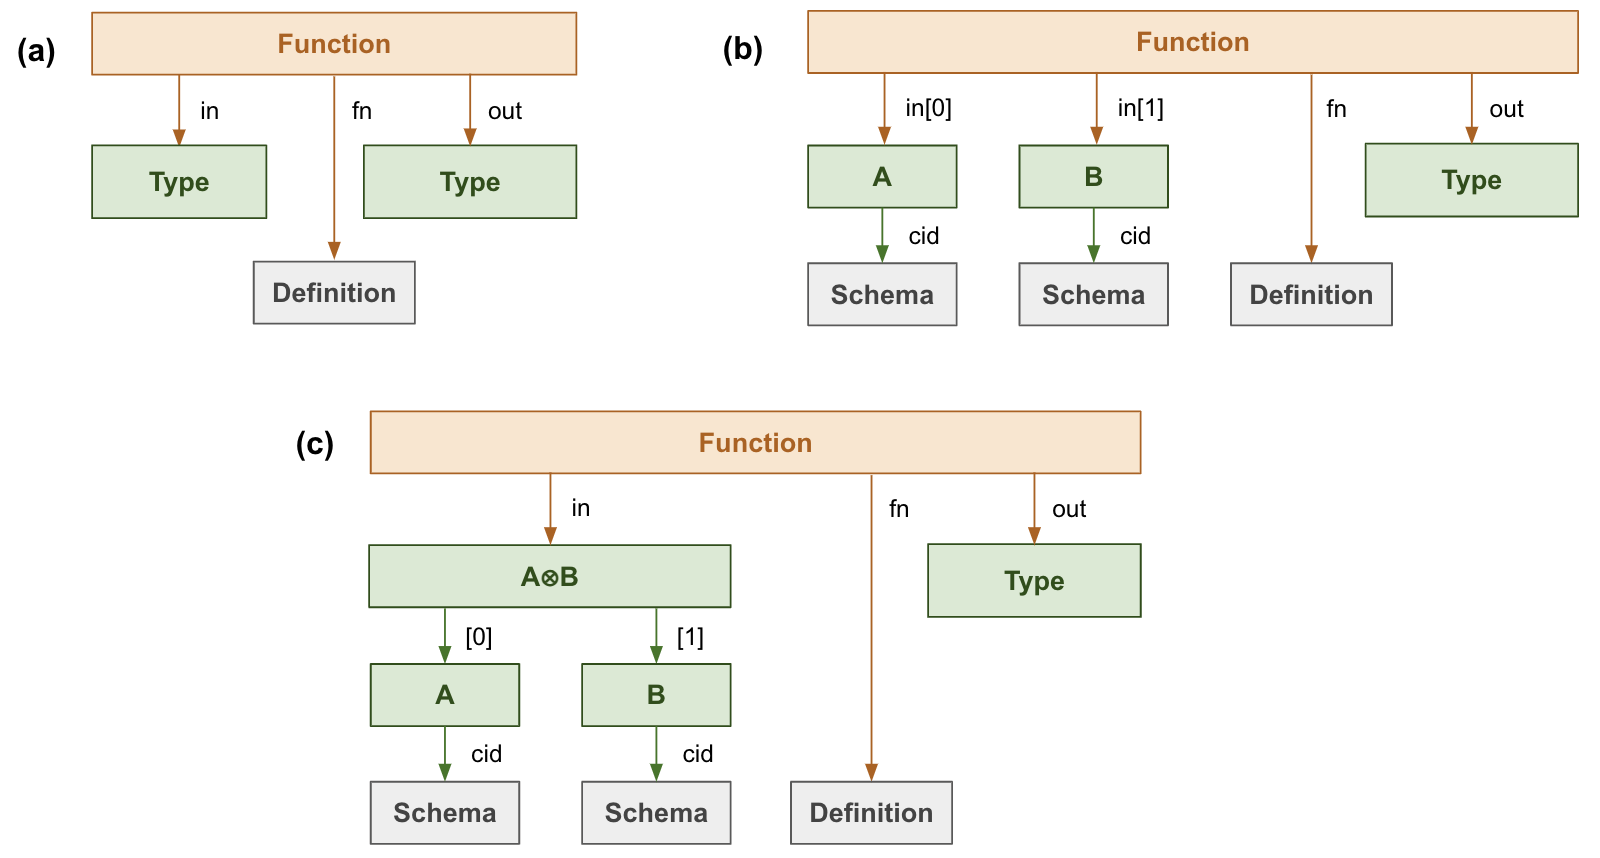
\includegraphics[width=1\columnwidth]{fig_functions}
\captionof{figure}[Functions]{Block diagram showing functions in Transform.Storage. (a) A function consists of input and output types, as well as a function definition which accepts data conforming to the given input types and returns data conforming to the given output types. (b) A function accepting the series type $A \otimes B$, in which this input type is represented in normal form. (c) A function with the same series input as $b$, where this input is represented in non-normal form.}
\label{functions_fig}
\end{center}
\setlength{\parindent}{.5 cm}

\subsection{Function}\label{function}
A function is an operation mapping from an input type to an output type. Functions themselves have types. If $f$ is a function mapping from type $A$ to type $B$, then $f : A \rightarrow B$ (``$f$ is of type $A$ to $B$"). A function in Transform.Storage contains information about the content addressed input and output types of that function, the function definition, and the execution environment in which the function was tested. These fields are shown in table \ref{functionFields}.
Values for $Function.execution$ and corresponding values for $Function.fn$ are given in the Execution Table (Table \ref{execTable}). The protocol includes a set of built-in functions, which correspond to fundamental operations on a computational graph, as well as the ability to externally define functions.

The height of a function is defined as $Max( Function.in.height, Function.out.height )$.




\begin{center}
\begin{tabular}{ || p{5cm} | p{9cm} ||}
\hline			
\multicolumn{2}{|| l ||}{\textbf{Function Fields}} \\
\hline
\makecell[l]{\textbf{execution} \\ \textit{(string)}} & \makecell[l]{Value chosen from the execution table. Necessary to \\ interpret fn.} \\
\hline
\makecell[l]{\textbf{fn} \\ \textit{(See Table \ref{execTable})}} & \makecell[l]{Function definition of type chosen from the Execution \\ Table}\\
\hline
\makecell[l]{\textbf{reference} \\ \textit{(string)}} & \makecell[l]{Pointer (CID or URL) to human-readable $fn$ code. Not \\ used in execution.} \\
\hline
\makecell[l]{\textbf{in} \\ \textit{(type)}} & \makecell[l]{Input type. May be a CID, an IPLD object or an IPLD \\ array.} \\
\hline
\makecell[l]{\textbf{out} \\ \textit{(type)}} & \makecell[l]{Output type. May be a CID, an IPLD object or an IPLD \\ array.} \\
\hline
\makecell[l]{\textbf{environment} \\ \textit{(string)}} & \makecell[l]{Compute environment where this function was tested, \\ chosen from the environment table} \\
\hline
\makecell[l]{\textbf{env\_params} \\ \textit{(string)}} & \makecell[l]{Parameters passed to the environment. Format depends \\ on the value of environment.} \\
\hline
\makecell[l]{\textbf{creator} \\ \textit{(string)}} & \makecell[l]{The public identifier of the creator of this type} \\
\hline
\makecell[l]{\textbf{creator\_id\_format} \\ \textit{(string, required if Type.creator} \\ \textit{is non-null})} & \makecell[l]{Value from the Identifier Table (section \ref{transformID}) describing \\ the type of identifier associated with the creator \\ field}\\
\hline
\makecell[l]{\textbf{protocol\_name} \\ \textit{(string)}} & \makecell[l]{Must be ``transform.storage"} \\
\hline
\makecell[l]{\textbf{protocol\_version} \\ \textit{(string)}} & \makecell[l]{The version of the protocol which this type is pursuant \\ to, such as  ``2.0.0"} \\
\hline			
\makecell[l]{\textbf{name} \\ \textit{(string, optional)}} & \makecell[l]{Short human-readable label} \\
\hline
\makecell[l]{\textbf{description} \\ \textit{(string, optional)}} &\makecell[l]{ Longer human-readable label}  \\
\hline  
\end{tabular}
\end{center}
\captionof{table}[Function Fields]{Definitions of the canonical fields describing a Transform.Storage function.}
\label{functionFields}
\setlength{\parindent}{.5 cm}
\vspace{.25 cm}




\begin{center}
\begin{tabular}{ || p{3cm} | p{3cm} | p{5.5cm} | p{4.5cm} ||}
\hline
\makecell[c]{\textbf{execution}} & \makecell[c]{\textbf{fn}} & \makecell[c]{\textbf{Description}}  & \makecell[c]{\textbf{Image}}  \\
\hline
\makecell[l]{identity} & \makecell[l]{null} & \makecell[c]{$f(x) = x$}  & \makecell[c]{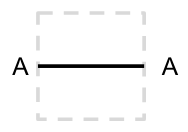
\includegraphics[width=.1\columnwidth]{builtInFns_id}}  \\
\hline
\vspace{.1 cm} \makecell[l]{introduce} & \vspace{.1 cm} \makecell[l]{CID of a type} & \vspace{0 cm} \makecell[c]{$f(null) = x$ in order to introduce $x$ \\as a constant.}  & \vspace{-0.2 cm} \makecell[c]{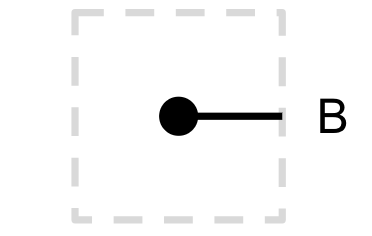
\includegraphics[width=.1\columnwidth]{builtInFns_introduce}} \vspace{0 cm} \\
\hline
\vspace{.1 cm}  \makecell[l]{ignore} & \vspace{.1 cm}  \makecell[l]{null} & \vspace{0 cm} \makecell[c]{$f(x) = null$ drop $x$ \\from the computational graph.}  & \vspace{-0.2 cm} \makecell[c]{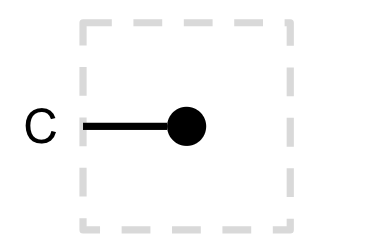
\includegraphics[width=.1\columnwidth]{builtInFns_ignore}}  \\
\hline
\end{tabular}
\end{center}

\begin{center}
\begin{tabular}{ || p{3cm} | p{3cm} | p{5.5cm} | p{4.5cm} ||}
\hline
\makecell[c]{\textbf{execution cont'd}} & \makecell[c]{\textbf{fn cont'd}} & \makecell[c]{\textbf{Description cont'd}}  & \makecell[c]{\textbf{Image cont'd}}  \\
\hline
\vspace{1.2 cm}  \makecell[l]{down} &  \vspace{1.2 cm} \makecell[l]{null} & \vspace{.7 cm} \makecell[c]{ $f(D\otimes null... \otimes null) = $ \\ $ null ... \otimes null \otimes D$ \\Shifts input down n+1 rows. \\ Height = n+2.}  & \vspace{-0.2 cm} \makecell[c]{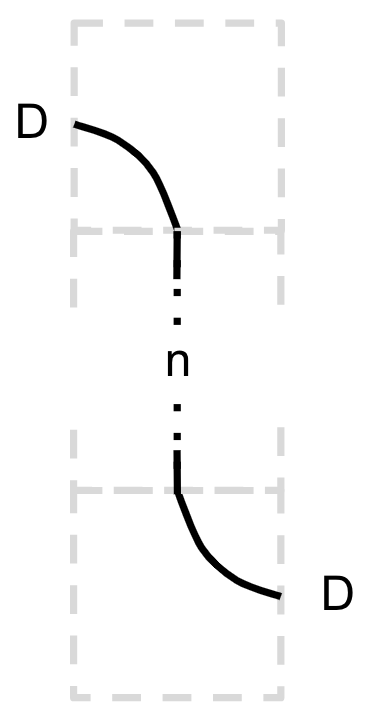
\includegraphics[width=.1\columnwidth]{builtInFns_down}}  \\
\hline
\makecell[l]{up} & \makecell[l]{null} & \makecell[c]{ $f(null... \otimes null \otimes E) = $ \\ $ E\otimes null ... \otimes null $ \\Shifts input down n+1 rows. \\ Height = n+2.}  & \makecell[c]{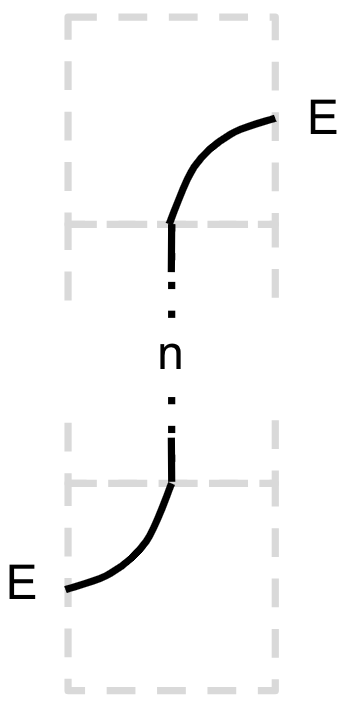
\includegraphics[width=.1\columnwidth]{builtInFns_up}}  \\
\hline
\makecell[l]{duplicate down} & \makecell[l]{null} & \makecell[c]{ $f(F\otimes null) = F\otimes F$ \\ Duplicates input.}  & \makecell[c]{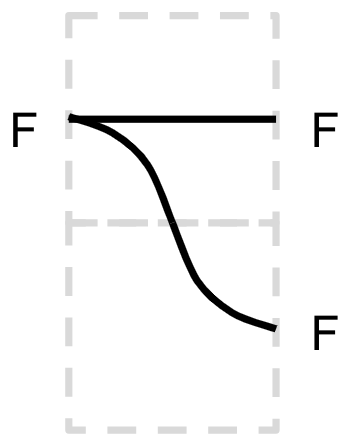
\includegraphics[width=.1\columnwidth]{builtInFns_dupDown}}  \\
\hline
\makecell[l]{duplicate up} & \makecell[l]{null} & \makecell[c]{ $f(null \otimes G) = G\otimes G$ \\ Duplicates input.}  & \makecell[c]{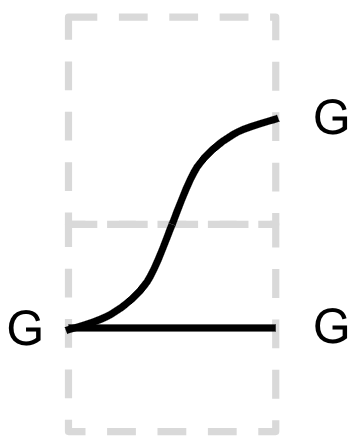
\includegraphics[width=.1\columnwidth]{builtInFns_dupUp}}  \\
\hline
\vspace{.6 cm} \makecell[l]{braid} & \vspace{.6 cm} \makecell[l]{null} & \vspace{.4 cm} \makecell[c]{ $f(H \otimes I) = I\otimes H$ \\ Switches the order of two inputs.}  & \vspace{-0.2 cm} \makecell[c]{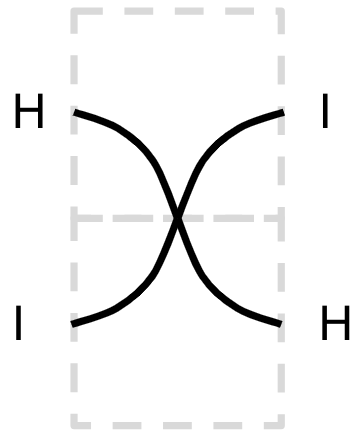
\includegraphics[width=.1\columnwidth]{builtInFns_braid}}  \\
\hline
\makecell[l]{WASM} & \makecell[l]{CID of WASM \\ function} & \makecell[c]{ $f(J) = K$ \\ Runs function on input J to \\ produce output K. J and/or \\ K may be a series type.}  & \makecell[c]{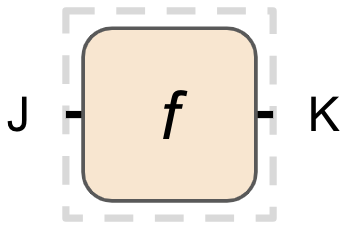
\includegraphics[width=.1\columnwidth]{builtInFns_function}}  \\
\hline
\makecell[l]{IPDR} & \makecell[l]{CID of IPDR \\ docker image} & \makecell[c]{ $f(J) = K$ \\ Runs function on input J to \\ produce output K. J and/or \\ K may be a series type.}  & \makecell[c]{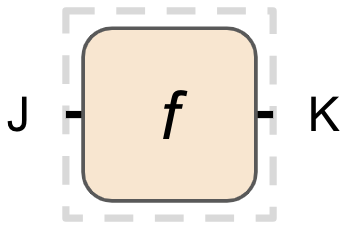
\includegraphics[width=.1\columnwidth]{builtInFns_function}}  \\
\hline
\makecell[l]{pipeline} & \makecell[l]{CID of a pipeline} & \makecell[c]{ $pipeline(L) = M$ \\ Executes function pipeline on input.}  & \makecell[c]{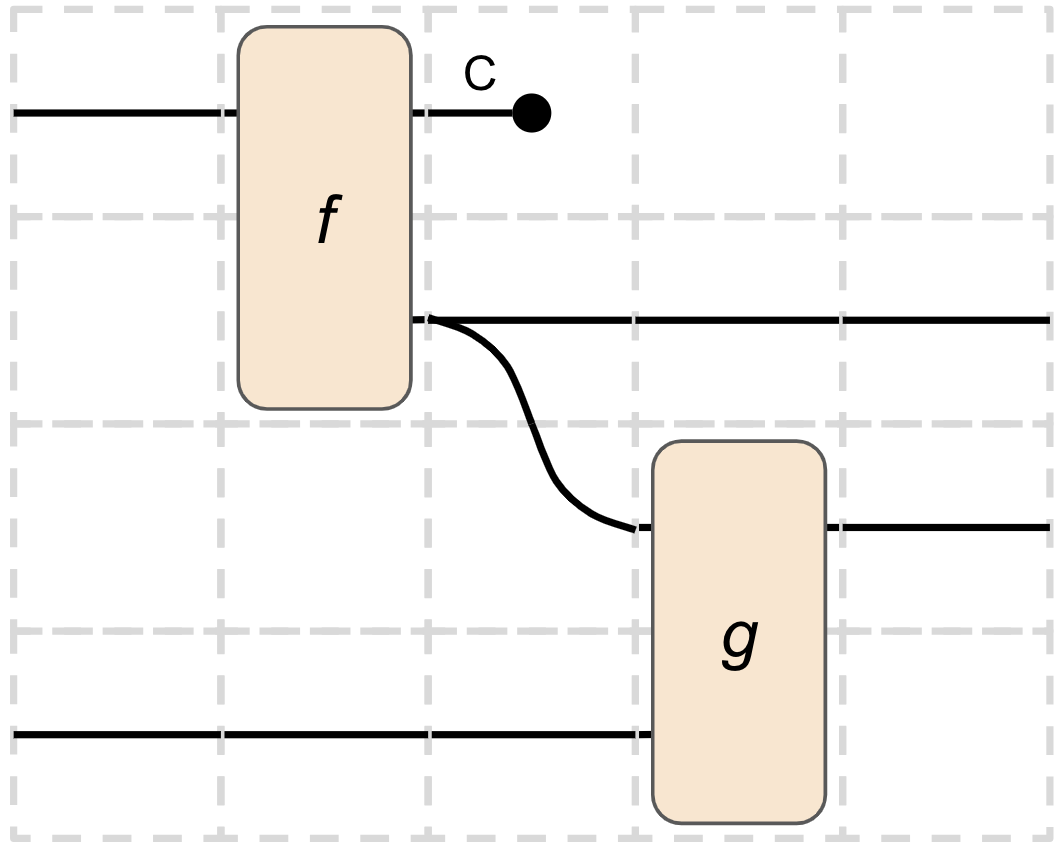
\includegraphics[width=.1\columnwidth]{builtInFns_pipeline}}  \\
\hline
\end{tabular}
\end{center}
\captionof{table}[Execution Table]{Execution Table. The function definition (Table \ref{functionFields} includes $fn$ and $execution$ variables defining functions and how they are interpreted. In the case of functions built in to Transform.Storage such as $identity$ or $introduce$, the $execution$ variable determines the identity of the function parameterized by $fn$. In the case of an externally defined function, $fn$ is a pointer to the function and $execution$ parameterizes the interpretation of this function.}
\label{execTable}
\setlength{\parindent}{.5 cm}

\vspace{.25 cm}

\subsection{Non-Interference}\label{nonInterference}
The type structure outlined here follows the principle of non-interference: \textit{every layer only references layers below it, never above it.} Thus, data never makes assumptions about type, type does not make assumptions about functions, and no lower level makes assumptions about provenance. This is necessary to ensure interoperability: higher levels are always extensible to include new lower-level cases as long as they can be referenced unambiguously using content addresses. 


\section{Functionality}\label{pseudocode}

This section contains pseudocode for functionality in implementations of transform.storage.

\subsection{Transform.Storage Data Model Required Functions}\label{dataModelFuncs}

Functionality required in any implementation of transform.storage. While these functions respect the logical equivalence between data structures and the CIDs of these data structures, they interoperate between the two on a `best effort' basis. Some implementations of transform.storage may not have access to a live IPFS node (example: if the implementation itself is on-chain), they may be offline, or the required CID may not be retrievable.

In addition to the result, functions return an error code and documentation of the implementation version of the function. Functions below are labeled with the protocol version described.

\subsubsection{isSimpleTypeNormalForm 2.0.0}\label{isSimpleTypeNormalForm_code}

Accepts a type. Result is a boolean which is true if the input argument is a simple type (ie. not a series type) and is in the normal form.

Protocol implementation maintains $isSimpleTypeNormalForm.version$ : $Str$, and  and array of supported $Type.protocol\_version$ values.

\vspace{.25 cm}
\begin{algorithm}[H]
\setcounter{AlgoLine}{0}
\caption{\textbf{isSimpleTypeNormalForm : \\ $Type \rightarrow \{result: Boolean, code: Str, protocol: ``transform.storage", protocol\_version : Str\}$}}
\label{algo_isSimpleTypeNormalForm}
\SetKwInOut{Input}{input}
\SetKwBlock{Begin}{Begin}{}
\Input{Type $T$}
\label{alg:quad}
\SetAlgoLined
$suffix$ $\leftarrow$ \{protocol: ``transform.storage", protocol\_version : isSimpleTypeNormalForm.version\} \\
\uIf{T is $True$} {
	\tcc{$True$ is a valid simple type}
	\Return \{result: $True$, code: $null$, ...$suffix$\}
	}
\uElseIf{T is $False$} 
{
	\tcc{$False$ is a valid simple type}
	\Return \{result: $False$, code: ``Type T is False", ...$suffix$\}
}
\uElseIf{T is an object}
{
	\uIf{T does not have a key $T.protocol$ with value ``Transform.Storage"}
		{\Return \{result: $False$, code: ``Type T does not use the Transform.Storage protocol", ...$suffix$\}}
	\uElseIf{T does not have a key $T.protocol\_version$}
		{\Return \{result: $False$, code: ``Type T does not list a Transform.Storage protocol version", ...$suffix$\}}
	\uElseIf{$T.protocol\_version$ is not supported}
		{\Return \{result: $False$, code: ``Type T uses Transform.Storage protocol version " + $T.protocol\_version$ + `` not supported by this implementation", ...$suffix$\}}
	\uElseIf{T does not have all the canonical fields for the given protocol version (see table \ref{typeFields})}
		{\Return \{result: $False$, code: `T does not contain required Type fields for transform.storage version " + $T.protocol\_version$, ...$suffix$\}}
	\tcc{If T is an object with the required fields of a supported transform.storage version, then it is a valid simple type in the normal form.}
	\Else{\Return \{result: $True$, code: $null$, ...$suffix$\}}
}
\Else{
	\Return \{result: $False$, code: ``T is not an object", ...$suffix$\}
}
\end{algorithm}


\subsubsection{normalizeType 2.0.0}\label{normalizeType_code}

Accepts a type. Returns the normal form of that type, a boolean indicating whether normalization was successful, and an error code. This function also serves to determine whether an input argument is a valid type.

Protocol implementation maintains $normalizeType.version$ : $Str$, and an array of supported versions of $isSimpleTypeNormalForm$.

\vspace{.25 cm}
\begin{algorithm}[H]
\setcounter{AlgoLine}{0}
\caption{\textbf{normalizeType : \\ $Type \rightarrow \{result: Type, success: Boolean, code: Str, protocol: ``transform.storage", protocol\_version : Str\}$}}
\label{algo_isSimpleTypeNormalForm}
\SetKwInOut{Input}{input}
\SetKwBlock{Begin}{Begin}{}
\Input{Type $T$}
\label{alg:quad}
\SetAlgoLined
$suffix$ $\leftarrow$ \{protocol: ``transform.storage", protocol\_version : normalizeType.version\} \\
alreadySimpleNormal $\leftarrow$ isSimpleTypeNormalForm(T)\\
\uIf{alreadySimpleNormal.protocol\_version not supported}{
				\Return \{result: null, success: $False$, code: ``isSimpleTypeNormalForm version" + alreadyNormal.protocol\_version + `` not supported by normalizeType version " + ``normalizeType.version", ...$suffix$\}
}
\uElseIf{isSimpleTypeNormalForm(T).result is $True$}{
	\tcc{If T is a simple type in its normal form, then it is already normalized}
	\Return \{result: T, success: $True$, code: $null$, ...$suffix$\}
}
\uElseIf{T is a CID}{
	\uIf{Have IPFS node}{
		\tcc{If T is a CID and this implementation has access to an IPFS node, expand the CID and run recursively.}
		$T_{Expanded} \leftarrow$ Retrieve $T$ from IPFS\\
		\Return normalizeType($T_{Expanded}$)
	}
	\Else{
		\Return  \{result: null, success: $False$, code: ``Could not expand CID", ...$suffix$\}
		}
}
\uElseIf{T is an array}{
	\tcc{If T is an array, then normalize each element of the array}
	toReturn $\leftarrow$ [ ] \\
	\For{index i of T}{
		elemResult $\leftarrow$ normalizeType($T[i]$)\\
		\uIf{elemResult.success is $False$}{
			\Return elemResult
		}
		\Else{
			\tcc{If we successfully normalized $T[i]$ then add to toReturn either by concatenating (if the normalized form is an array) or appending.}
			\uIf{elemResult.result is an array}{
				toReturn $\leftarrow$ Concatenate toReturn and elemResult.result
				}
			\Else{
				toReturn $\leftarrow$ toReturn + elemResult.result
			}
		}
	}
	\Return \{result: toReturn, success: $True$, code: $null$, ...$suffix$\}
}
\Else{
	\tcc{If T were a simple type, it would either be a CID or in its normal form. If T were a series type, it would either be a CID or an array. Therefore, at this point in the code T must not be a valid type.}
	\Return  \{result: null, success: $False$, code: ``T is not a type", ...$suffix$\}
}

\end{algorithm}


\subsubsection{isTerm 2.0.0}\label{isTerm_code}

Accepts a type in its normal form, and a data blob. Returns a boolean which is true if the protocol implementation could determine that data is a valid term of the given type, and false otherwise; and an error code.

Protocol implementation maintains $isTerm.version$ : $Str$, and array of supported $Type.protocol\_version$ values.

\vspace{.25 cm}
\begin{algorithm}[H]
\setcounter{AlgoLine}{0}
\caption{\textbf{isTerm : \\ $(Type \otimes Data) \rightarrow \{result: Boolean, code: Str, protocol: ``transform.storage", protocol\_version : Str\}$}}
\label{algo_isTerm}
\SetKwInOut{Input}{input}
\SetKwBlock{Begin}{Begin}{}
\Input{Type $T$, Data $D$}
\label{alg:quad}
\SetAlgoLined
$suffix$ $\leftarrow$ \{protocol: ``transform.storage", protocol\_version : isTerm.version\} \\
\tcc{Check for special cases $True$ and $False$}
\uIf{T is $True$} {
	\tcc{Every data blob D is a valid term of type True}
	\Return \{result: $True$, code: $null$, ...$suffix$\}
	}
\uElseIf{T is $False$} 
{
	\tcc{Type $False$ has no terms}
	\Return \{result: $False$, code: ``Type T is False", ...$suffix$\}
}
\tcc{If this is a simple type}
\uElseIf{T is an object}
	{
		\tcc{T must be a simple type}
		\If{T.protocol is not ``Transform.Storage"}{\Return \{result: $False$, code: ``Type T does not use the Transform.Storage protocol", ...$suffix$\}}
		\If{T.protocol\_version is not supported}{\Return \{result: $False$, code: ``Type T uses Transform.Storage protocol version " + $T.protocol\_version$ + `` not supported by this implementation", ...$suffix$\}}
		Using the type checking table from the version of the protocol indicated by $T.protocol\_version$, look up $T.type\_checking$ to determine the type checking function $f_{check}$\\
    		\Return \{...$f_{check}(T, D)$, ...$suffix$\}
	}
\tcc{If this is a series type}
\uElseIf{T is an array} 
{
	\If {D is not array with the same length as T}
	{
		\Return \{result: $False$, code: ``D and T length mismatch", ...$suffix$\}
	}
	\For{index i of T}{
		\tcc{T and D are both arrays of the same length, so run recursively on each pair of elements}
		\If {isTerm(T[i], D[i]) returns false}
		{\Return \{result: $False$, code: ``D and T mismatch at index " + i, ...$suffix$\}}
	\tcc{At this point in the code, each element of must T match the corresponding element of D}
	\Return \{result: $True$, code: $null$, ...$suffix$\} \\
  }
    }
\Else
{
	\tcc{T is not in the correct format}
	\Return \{result: $False$, code: ``T is not the normal form of a transform.storage type" , ...$suffix$\}\
}
\end{algorithm}



\subsubsection{isValidAsset 2.0.0}\label{isValidAsset_code}

Accepts an asset. Result is true if the protocol implementation could determine that the asset is valid, and false otherwise. Retrieves asset payload CIDs non-recursively, as discussed in section \ref{asset}.

Protocol implementation maintains $isValidAsset.version$ : $Str$, and arrays of supported $Asset.protocol\_version$, $isSimpleTypeNormalForm$, and $isTerm$ values.

\vspace{.25 cm}
\begin{algorithm}[H]
\setcounter{AlgoLine}{0}
\caption{\textbf{isValidAsset : \\ $Asset \rightarrow \{result: Boolean, code: Str, protocol: ``transform.storage", protocol\_version : Str\}$}}
\label{algo_isValidAsset}
\SetKwInOut{Input}{input}
\SetKwBlock{Begin}{Begin}{}
\Input{Asset $A$}
\SetAlgoLined
$suffix$ $\leftarrow$ \{protocol: ``transform.storage", protocol\_version : $isValidAsset.version$\} \\
\tcc{If A is the CID of an Asset and this implementation has access to an IPFS node, expand the CID and run recursively.}
\uIf{A is a CID}{
	\uIf{Have IPFS node}{
		$A_{Expanded} \leftarrow$ Retrieve $A$ from IPFS\\
		\Return isValidAsset($A_{Expanded}$)
	}
	\Else{
		\Return  \{result: $False$, code: ``Could not expand CID", ...$suffix$\}
		}
}
\tcc{If A is an object, evaluate it.}
\uIf{A is an object}
{
	\uIf{A does not have a key $A.protocol$ with value ``Transform.Storage"}
		{\Return \{result: $False$, code: ``Asset A does not use the Transform.Storage protocol", ...$suffix$\}}
	\uElseIf{A does not have a key $A.protocol\_version$}
		{\Return \{result: $False$, code: ``Asset A does not list a Transform.Storage protocol version", ...$suffix$\}}
	\uElseIf{$A.protocol\_version$ is not supported}
		{\Return \{result: $False$, code: ``Asset A uses Transform.Storage protocol version " + $A.protocol\_version$ + `` not supported by this implementation", ...$suffix$\}}
	\uElseIf{A does not have all the canonical fields for the given protocol version (see table \ref{assetFields})}
		{\Return \{result: $False$, code: ``A does not contain required Asset fields for transform.storage version " + $A.protocol\_version$, ...$suffix$\}}
		}
\uElse{
		\tcc{A is an object with the correct fields, so evaluate whether A.payload is a term of A.template.}
		normalizedTemplate $\leftarrow$ normalizeType(A.template)\\
		\uIf{normalizedTemplate.protocol\_version not supported}{
				\Return \{result: $False$, code: ``normalizeType version" + normalizedTemplate.protocol\_version + `` not supported by isValidAsset version " + ``isValidAsset.version", ...$suffix$\}
		}
		\ElseIf{Not normalizedTemplate.success}{
			\Return \{result: $False$, code: normalizedTemplate.code, ...$suffix$\}
		}
		T $\leftarrow$ normalizedTemplate.result\\
}
\end{algorithm}
\textit{cont'd on next page}

\vspace{.25 cm}
\begin{algorithm}[H]
\setcounter{AlgoLine}{25}
\SetKwInOut{Input}{input}
\SetKwBlock{Begin}{Begin}{}
\SetAlgoLined
\nonl \contIndent{
	\nonl \contIndent{
		Initialize $D$\\
		\tcc{If A.payload is a CID, then retrieve it (exactly once, not recursively) to get the data referenced by the asset. In the edge case that the template schema describes a single CID, then this must be one hierarchical level down (ie. A.payload must be a CID of a CID).}
		\uIf{$A.payload$ is a CID}{
			\uIf{Have IPFS node}{
				$D \leftarrow$ Retrieve $A.payload$ from IPFS\\
			}
			\Else{
				\Return  \{result: $False$, code: ``Could not expand A.payload CID", ...$suffix$\}
			}
		}
		\tcc{In the case that both A.payload and T are arrays, this is a series payload. Expand every element of the payload if it is a CID, otherwise pass that element along unchanged.}
		\uElseIf{$A.payload$ is an array and T is an array}{
			$D \leftarrow$ [ ]\\
			\For{index i of A.payload}{
				\uIf{$A.payload[i]$ is a CID}{
					\uIf{Have IPFS node}{
						Retrieve $A.payload$ from IPFS and append to D\\
					}
					\Else{
						\Return  \{result: $False$, code: ``Could not expand A.payload[" + i + ``] CID", ...$suffix$\}
					}
				}
				\Else {Append $A.payload[i]$ to D}
			}
		}
		\tcc{If A.payload is not a CID and T and A.payload are not both arrays, pass A.payload along unchanged.}
		\Else{D $\leftarrow$ A.payload}
	}
	\textbf{end}\\
	\tcc{Evaluate whether D is a valid term of T}
	validTerm $\leftarrow$ isTerm(T, D)\\
	\Return \{result: validTerm.result, code: validTerm.code, ...$suffix$\}
}
\tcc{If A is neither a CID nor an object, it is not a valid Asset.}
\Else{
	\Return \{result: $False$, code: ``A is not an object", ...$suffix$\}
}
\end{algorithm}




\begin{center}
    
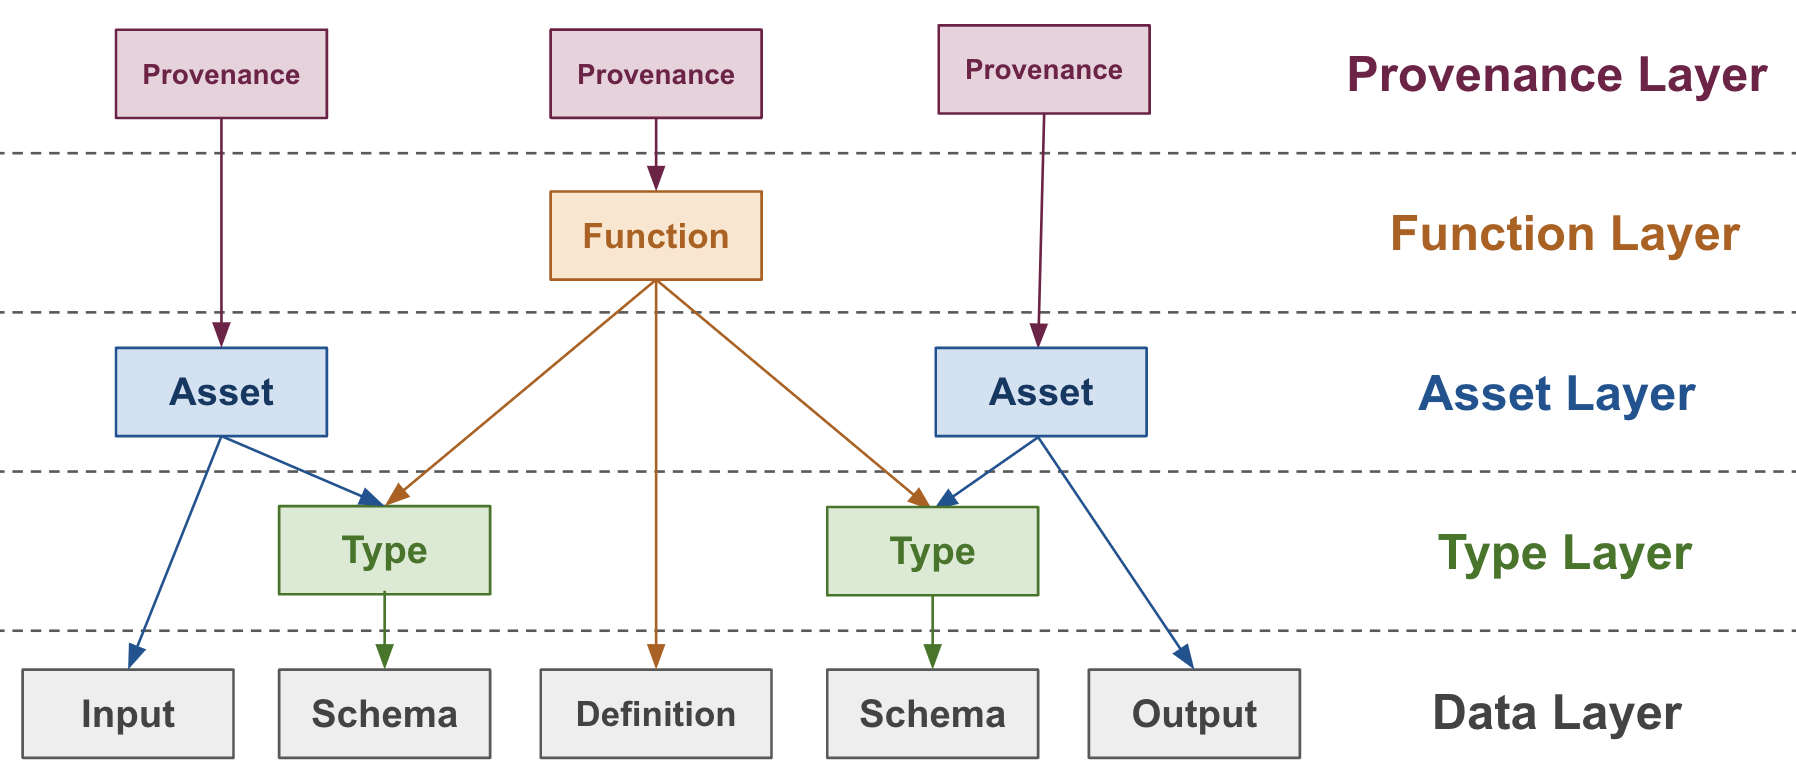
\includegraphics[width=1\columnwidth]{pipeline_layers_20230715}
\captionof{figure}[Simple compute pipeline]{Diagram of a simple compute pipeline consisting of one input asset, one function, and one output asset highlighting relationships between data model components.}
\label{simplePipeline}
\end{center}


% the bibliography file (below) needs to have the same name as the tex file
% run typeset .tex file as LaTeX, then typeset .bib file as BibTeX, then twice typeset .tex as LaTeX
\bibliography{transform-prov-paper}{}
\bibliographystyle{plain}


\end{document}  

